\documentclass[11pt]{article}
\usepackage[margin=1in]{geometry}
\usepackage{booktabs}
\usepackage{amsmath}
\usepackage{xcolor}
\usepackage{tikz}
\usepackage[colorlinks=true,linkcolor=blue,urlcolor=blue]{hyperref}
\usepackage{enumitem}

\definecolor{good}{HTML}{2A9D4A}
\definecolor{bad}{HTML}{C0392B}
\definecolor{blu}{HTML}{2C6FBB}
\definecolor{gry}{HTML}{888888}

\title{\vspace{-1.2cm}\textbf{Cascade-Direction Inference on a T-cell Maturation Axis}\\[2pt]
\large A recovered timeline, a clean reversal, and a falsified hypothesis}
\author{cytokine-MIL project (\S32) \quad\textemdash\quad session summary}
\date{2026-06-22}

\begin{document}
\maketitle
\vspace{-1.0cm}

\begin{abstract}
\noindent We extended the validated \texttt{cross\_asym} cascade-\emph{direction} statistic to a
\textbf{T-cell maturation} axis (naive$\rightarrow$effector$\rightarrow$memory) on a public
SARS-CoV-2 vaccination whole-PBMC CITE-seq atlas. The method \textbf{recovers the vaccination
\emph{timeline}} (D2$\rightarrow$D11$\rightarrow$D28) from one cross-sectional snapshot, but
\textbf{exactly \emph{reverses} the differentiation \emph{state} order}. A control-swap
decomposition shows the reversal is \emph{control-independent} and \textbf{falsifies our own
first-pass explanation}. The insight: \texttt{cross\_asym} reads a program-\emph{acquisition}
asymmetry while differentiation is a program-\emph{retention} asymmetry --- so it is correctly
signed on a temporal/progression axis but mis-signed on a cell-state axis.
\end{abstract}

\section{Setup}
The direction statistic, for an ordered pair $(a,b)$ with per-condition discovered signatures
$S_a,S_b$ and a control population, is
\begin{equation}
\mathrm{cross\_asym}(a,b)=\underbrace{\big[s(a,S_b)-s(b,S_a)\big]}_{\text{raw cross-engagement (b)}}
-\underbrace{\big[\mathrm{ctrl}_{S_b}-\mathrm{ctrl}_{S_a}\big]}_{\text{control term (a)}},
\label{eq:cross}
\end{equation}
where $s(x,S)$ is the mean expression of gene set $S$ in population $x$. The biology it encodes:
an \emph{upstream} stimulus's cells carry \emph{both} their own and the (autocrine)
\emph{downstream} program, so $s(\text{up},S_{\text{down}})>s(\text{down},S_{\text{up}})$.

\paragraph{Experiment.} Dataset: multimodal SARS-CoV-2 vaccination atlas (\emph{Nat.\ Immunol.}
2023; Zenodo \texttt{7555405}, no-auth). Whole-PBMC CITE-seq, days 0/2/11/28, 6 donors,
61{,}911 T cells. We reused the \S30 disease-progression pipeline verbatim and ran two framings:
\textbf{(i) STATE} --- condition $=$ maturation state \{Naive, Effector, Memory\} from CITE
\emph{surface protein} gating (CD45RO/CD27; RNA-independent, so state labels cannot leak into
the RNA signatures), control $=$ day-0 ``Resting''; and \textbf{(ii) TIMEPOINT} --- condition
$=$ \{D2, D11, D28\}, control $=$ D0. An independent synthetic \emph{apparatus} provides a
distinct-program go/no-go gate.

\section{Results: a recovered timeline and a reversed state order}
The three framings give a sharp, internally-consistent picture (Table~\ref{tab:main}): the
apparatus passes its hard gate, the \emph{timeline} direction is recovered perfectly, and the
\emph{state} direction is exactly inverted. The tell-tale is the relationship between the
direction statistic and its symmetric control (Fig.~\ref{fig:bars}): on the apparatus and
timepoint axes \texttt{cross\_asym} $\gg$ \texttt{directional\_score}, but on the state axis the
two \emph{swap} (control $100\%$, direction $0\%$) --- the ``no-seed/monotone'' regime the
apparatus reproduces synthetically.

\begin{table}[h]
\centering
\small
\begin{tabular}{lcccl}
\toprule
framing & \texttt{cross\_asym} acc. & symm.\ control & Kendall $\tau$ & verdict \\
\midrule
Apparatus (distinct-program gate) & $100\%$ & $50\%$ & $+1.0$ & \textcolor{good}{PASS} \\
\textbf{Timepoint} D2$<$D11$<$D28 & $\mathbf{100\%}$ & $0\%$ & $\mathbf{+1.0}$ & \textcolor{orange}{AMBER}$^\dagger$ \\
\textbf{State} Naive$<$Eff$<$Mem & $\mathbf{0\%}$ & $100\%$ & $\mathbf{-1.0}$ & \textcolor{bad}{RED (reversed)} \\
\bottomrule
\end{tabular}
\caption{Direction recovery under the two real framings plus the synthetic gate.
$^\dagger$Timepoint is AMBER \emph{only} because the 6-donor bootstrap CI is wide
($[0.33,1.0]$); the point estimate is perfect. Recovered orders: timepoint
$=$ D2$\rightarrow$D11$\rightarrow$D28 (truth); state $=$
Memory$\rightarrow$Effector$\rightarrow$Naive (the exact reverse of truth, hence $\tau=-1.0$).}
\label{tab:main}
\end{table}

\begin{figure}[h]
\centering
\scalebox{0.84}{%
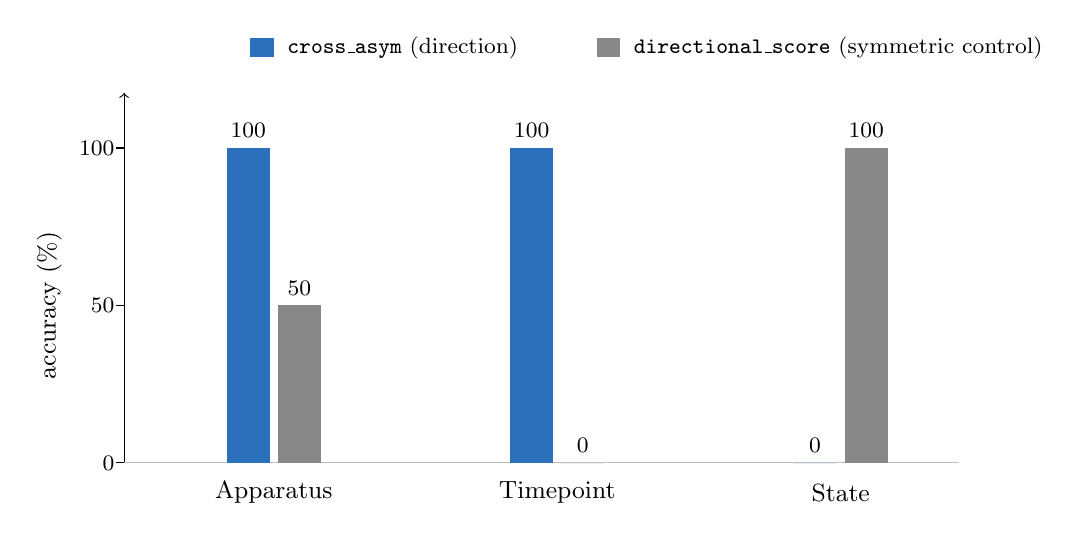
\begin{tikzpicture}
% y-axis 0..100 -> 0..4 cm ; legend on top
\draw[->] (0,0) -- (0,4.7);
\node[rotate=90,font=\small] at (-0.95,2.0) {accuracy (\%)};
\foreach \p/\y in {0/0, 50/2.0, 100/4.0} {\draw (-0.1,\y)--(0,\y) node[left,font=\footnotesize]{\p};}
\draw[gray!50] (0,0) -- (10.6,0);
% Apparatus (cx~1.9), Timepoint (cx~5.5), State (cx~9.1): cross=blu, control=gry
\fill[blu] (1.30,0) rectangle (1.85,4.00); \node[font=\footnotesize] at (1.575,4.22){100};
\fill[gry] (1.95,0) rectangle (2.50,2.00); \node[font=\footnotesize] at (2.225,2.22){50};
\node[font=\small] at (1.90,-0.38){Apparatus};
\fill[blu] (4.90,0) rectangle (5.45,4.00); \node[font=\footnotesize] at (5.175,4.22){100};
\fill[gry] (5.55,0) rectangle (6.10,0.00); \node[font=\footnotesize] at (5.825,0.22){0};
\node[font=\small] at (5.50,-0.38){Timepoint};
\fill[blu] (8.50,0) rectangle (9.05,0.00); \node[font=\footnotesize] at (8.775,0.22){0};
\fill[gry] (9.15,0) rectangle (9.70,4.00); \node[font=\footnotesize] at (9.425,4.22){100};
\node[font=\small] at (9.10,-0.38){State};
% legend
\fill[blu] (1.6,5.15) rectangle (1.9,5.4); \node[right,font=\footnotesize] at (1.95,5.27){\texttt{cross\_asym} (direction)};
\fill[gry] (6.0,5.15) rectangle (6.3,5.4); \node[right,font=\footnotesize] at (6.35,5.27){\texttt{directional\_score} (symmetric control)};
\end{tikzpicture}}
\caption{The ``inverse fingerprint.'' On the apparatus and timepoint axes the antisymmetric
direction statistic beats its symmetric control (the healthy cytokine/COVID pattern). On the
state axis the two swap places --- direction $0\%$, control $100\%$ --- the hallmark of an
axis where \texttt{cross\_asym}'s core assumption runs backwards.}
\label{fig:bars}
\end{figure}

\section{Anatomy of the reversal (and a falsified hypothesis)}
Our first-pass explanation was that the control (day-0 ``Resting'') $\approx$ Naive, so the
upstream state coincided with the baseline. To test it we ran a \textbf{control-swap
decomposition}: holding the discovered signatures \emph{fixed}, we varied only the control term
in Eq.~\eqref{eq:cross} --- including a \texttt{ZERO} control (no subtraction $=$ the raw
cross-engagement, i.e.\ effect (b) alone). Table~\ref{tab:decomp} and Fig.~\ref{fig:decomp} are
decisive: \textbf{the raw engagement is the \emph{most} inverted} ($+0.588$ vs $+0.140$ under
Resting), the control \emph{reduces} the inversion, and \emph{no} control choice un-inverts the
Naive pairs. The baseline-coincidence hypothesis is \textbf{falsified}: effect (a) mitigates,
it does not cause.

\begin{table}[h]
\centering
\small
\begin{tabular}{lccc}
\toprule
control & \texttt{cross\_asym}(Eff,Nai) & \texttt{cross\_asym}(Mem,Nai) & $\tau$ \\
\midrule
Resting (original)                 & $+0.107$ & $+0.140$ & $-1.0$ \\
\textbf{ZERO} $=$ raw engagement (b) & $\mathbf{+0.253}$ & $\mathbf{+0.588}$ & $-1.0$ \\
Balanced (removes naive/mem imbalance) & $+0.121$ & $+0.146$ & $-1.0$ \\
Naive as control                   & $+0.138$ & $+0.147$ & $-1.0$ \\
Memory as control                  & $+0.159$ & $+0.161$ & $-1.0$ \\
\bottomrule
\end{tabular}
\caption{Control-swap decomposition (\texttt{analyze\_vaccine\_state\_control\_decomp.py}).
The correct sign for an $X$--Naive pair is \emph{negative} (Naive upstream); every control
yields \emph{positive} (inverted). The raw cross-engagement (ZERO) is the most inverted, so the
inversion is intrinsic to the axis, not an artifact of the control.}
\label{tab:decomp}
\end{table}

\begin{figure}[h]
\centering
\scalebox{0.84}{%
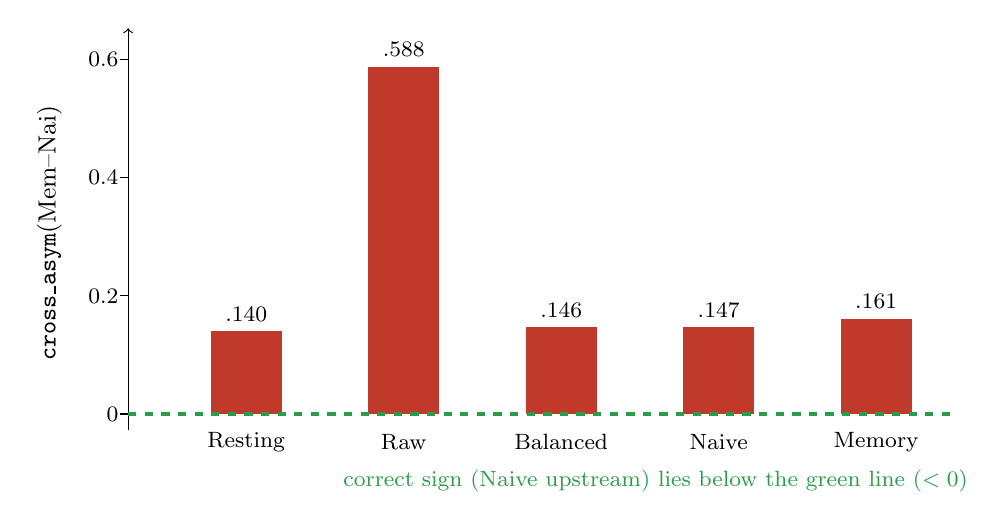
\begin{tikzpicture}
% y = value * 7.5 cm ; bars at x=1.5,3.5,5.5,7.5,9.5 (width 0.9)
\draw[->] (0,-0.2) -- (0,4.9);
\node[rotate=90,font=\small] at (-1.0,2.3) {\texttt{cross\_asym}(Mem--Nai)};
\foreach \v/\y in {0/0, 0.2/1.5, 0.4/3.0, 0.6/4.5} {\draw (-0.1,\y)--(0,\y) node[left,font=\footnotesize]{\v};}
\fill[bad] (1.05,0) rectangle (1.95,1.05); \node[font=\footnotesize] at (1.5,1.27){.140};
\fill[bad] (3.05,0) rectangle (3.95,4.41); \node[font=\footnotesize] at (3.5,4.63){.588};
\fill[bad] (5.05,0) rectangle (5.95,1.10); \node[font=\footnotesize] at (5.5,1.32){.146};
\fill[bad] (7.05,0) rectangle (7.95,1.10); \node[font=\footnotesize] at (7.5,1.32){.147};
\fill[bad] (9.05,0) rectangle (9.95,1.21); \node[font=\footnotesize] at (9.5,1.43){.161};
\foreach \x/\t in {1.5/Resting, 3.5/Raw, 5.5/Balanced, 7.5/Naive, 9.5/Memory}
  {\node[font=\footnotesize] at (\x,-0.35){\t};}
\draw[good,very thick,dashed] (0,0) -- (10.5,0);
\node[good,font=\footnotesize] at (6.7,-0.85){correct sign (Naive upstream) lies below the green line ($<0$)};
\end{tikzpicture}}
\caption{The inversion is control-independent. ``Raw'' is the \texttt{ZERO} control (no
normalization $=$ pure cross-engagement) and is the \emph{most} positive, i.e.\ most inverted;
every control keeps Memory above Naive. A genuine recovery would put these bars \emph{below}
the green line.}
\label{fig:decomp}
\end{figure}

\paragraph{The mechanism.} \texttt{cross\_asym} assumes program \emph{acquisition}: an upstream
cell \emph{gains} the downstream program (the cytokine-autocrine logic). Differentiation is the
opposite --- a program-\emph{retention} asymmetry: the \emph{mature} cell \emph{retains} the
\emph{progenitor's} program (memory T cells re-express the naive program: \textit{IL7R, TCF7,
SELL, CCR7}). Hence $s(\text{Memory},S_{\text{Naive}})\gg s(\text{Naive},S_{\text{Memory}})$ and
the statistic faithfully points mature$\rightarrow$naive. This is not a bug (the apparatus
distinct-gate passes) and not fixable by control choice; it is the method meeting an axis whose
biology is sign-flipped relative to its assumption.

\section{Takeaways}
\begin{itemize}[leftmargin=1.4em,itemsep=1pt]
\item \textbf{Boundary mapped.} \texttt{cross\_asym} direction transfers to \emph{temporal /
disease-progression} axes (vaccination timeline here; COVID severity in \S30) but is
fundamentally mis-signed on a \emph{cell-state differentiation} axis. The timeline is the right
axis for an acquisition-based statistic; recovering \emph{state} direction would need a
retention/loss-keyed statistic.
\item \textbf{Self-correction.} The control-swap decomposition falsified our own
baseline-coincidence explanation --- a reminder that the symmetric-control contrast and a raw
(no-control) ablation are the right tools to attribute a direction result.
\item \textbf{Engineering.} Staging the pipeline (inspect before GPU) caught three real schema
issues up front: the atlas samples \emph{Day 11} (not Day 10); obs fields are dotless
(\texttt{celltypel1/2}); and CCR7 is \emph{absent} from the panel, so state gating uses
CD45RO/CD27. The Seurat \texttt{.rds} was read without \texttt{SeuratObject} via base-R
\texttt{attr()} slot access (only \texttt{Matrix} required).
\item \textbf{Caveats.} Validation, not discovery (orders are textbook); cross-sectional
(direction, not forecast); \emph{early} (day-28) memory only; 6 donors (the bootstrap, not the
point estimate, is what limits the timepoint verdict to AMBER); direction $\neq$ causation.
\end{itemize}

\vspace{2pt}\noindent\footnotesize\textit{Sources:}
\texttt{reports/vaccine\_progression/} (\texttt{VACCINE\_PROGRESSION\_RESULTS},
\texttt{STATE\_CONTROL\_DECOMP}, \texttt{PRE\_REGISTRATION}); CLAUDE.md \S32; cluster jobs
30907134--38.
\end{document}
